\section*{Guidelines for Interpreting
Results}\label{guidelines-for-interpreting-results}

\emph{instructions: A brief discussion of the theory and applications of
your}

\emph{notes: Maybe mention how findings are relevant to the lab? For
example: Manually annotated content should be reliable, although one
should look at the `confidence' in the instance annotation. Predictions
are probably trustworthy, but you need to take into account the
`confidence score', and other features like whether its in a domain,
etc\ldots{}}

\section*{Commentary:}\label{commentary}

\emph{instructions: A brief discussion of the theory and applications of
your}

\subsection*{Background Information}\label{background-information}

In order to interpret the data contained in ELM and the results produced by the
ELM prediction tool, it is important to have a basic understanding of SLiM's
and how they are affected by their structural and biological context. This 
background information summarises the different functionalities of SLiMs, 
describes the degenerate nature of motif sequences, and emphasises the need for 
contextual data for confident SLiM prediction.

\subsubsection*{ELM categorises SLiMs depending on their functionality}

SLiMs mediate different types of interactions, and based on this functionality, 
the ELM classes annotated in the ELM database are grouped into six main ELM 
types (Figure 1) (\cite{24214962}). They can function as ligand binding sites or 
as sites for post-translational modification (PTM). Some ligand SLiMs are 
recognised by components of the cellular transport machinery and function as 
localisation signals that target proteins to specific sub-cellular compartments 
(TRG type). Other ligand SLiMs are abundantly present in interfaces that mediate 
the assembly of large macromolecular complexes and in highly modular scaffold 
proteins that act as multivalent platforms for protein complex assembly 
(LIG type). Docking motifs are ligand SLiMs that recruit modification enzymes to 
their substrates by binding to a site on the enzyme that is distinct from the 
active site (DOC type). A subset of these, known as degrons, recruit ubiquitin 
ligases, which subsequently polyubiquitylate their substrates and hence target 
them for proteasomal degradation (DEG type). SLiMs that act as sites for PTM can 
be targeted by specific enzymes for the addition or removal of a small chemical 
group (e.g. phosphorylation), a sugar molecule (e.g. glycosylation), a protein 
(e.g. ubiquitylation), or another moiety (e.g. lipidation) (MOD type). Other PTM 
SLiMs mediate proteolytic cleavage by acting as target site for proteolytic 
enzymes (CLV type), or are recognised for structural modification by isomerases 
that catalyse cis-trans isomerisation of the peptide backbone (DOC type) 
\cite{24926813, 24773235}.

\subsubsection*{ELM regular expressions reflect the degenerate nature of SLiMs}

As their name suggests, SLiMs are compact, being composed of a limited number of 
adjacent amino acids. Most of a motif’s binding specificity however is conferred 
by only a subset of these amino acids. Those few residues that directly interact 
with the binding partner are evolutionary conserved, although in many cases a 
subset of amino acids that share certain properties (such as similar charge, 
size or hydrophobicity) are allowed in these hotspot positions. In the motif 
positions that contribute little to the interaction, there are even less 
constraints, i.e. a broader range of amino acids is allowed in these positions 
\cite{21909575}. This sequence flexibility is captured in the regular 
expressions that are defined for each motif class. A first consequence of this 
degeneracy is that SLiMs co-operatively engage in interactions of relatively low 
affinity. Hence these binding events are transient and reversible, and can be 
readily modulated, for instance by PTM. These characteristics make SLiM-based 
interactions ideal mediators of the dynamic processes involved in cell 
signalling \cite{22480932}. Another consequence is that it might take only a few 
or even a single point mutation to generate or disrupt a functional motif in a 
protein. The associated ability to evolve convergently might underlie the 
proliferation of SLiMs and the rewiring of interactomes \cite{26589632,
22346764}. Conversely, several SLiM-associated diseases have been 
characterised to date, for instance Liddle syndrome \cite{15483078}.

\subsubsection*{ELM integrates data to increase the confidence of SLiM prediction*}

Due to their degenerate nature, motif sequences contain only very little 
information, and many short sequences in a proteome will match motif patterns. 
However, most of these matches will not represent functional motifs, and hence, 
when scanning a proteome for putative motifs using only the motif sequence 
patterns will yield a large number of false positive instances, far exceeding 
the number of true motifs. Therefore, reliable motif detection cannot go without 
experimental validation of candidate motifs, using different types of 
experiments and techniques \cite{26581338}. This however does not mean that 
bioinformatics analysis cannot guide researchers towards a subset of candidate 
motifs that have a higher probability to be functional and help rule out those 
candidate motifs that are likely to be false positives. Taking into account 
additional information, besides a match to a sequence pattern defining a SLiM, 
can greatly narrow the selection of putative motifs for experimental validation. 
Additional data for in silico analysis include conservation of the motif 
sequence, the location of the motif within the protein’s structure and its 
accessibility for its binding partner, validated interaction with the binding 
partner, and in-cell co-localisation with the binding partner. The availability 
and usefulness of these additional data for SLiM discovery depends on their 
extensive and correct biocuration. A vast and increasing amount of biological 
data is available in a wide variety of sources, including the literature and 
large-scale datasets. In order to facilitate integration of data, they need to 
be collected, annotated and formatted in central data and knowledge 
repositories. The ELM database provides such a repository for experimentally 
validated linear motif classes and instances. The ELM prediction tool in turn 
relies on annotated data, both from the ELM database and other resources, to 
accurately analyse unknown sequences for candidate motifs and assist researchers 
in selecting the most plausible ones for experimental validation and discard 
likely false positive hits, saving them valuable time and assets 
\cite{22110040}.

\begin{figure}[h!]
\centering
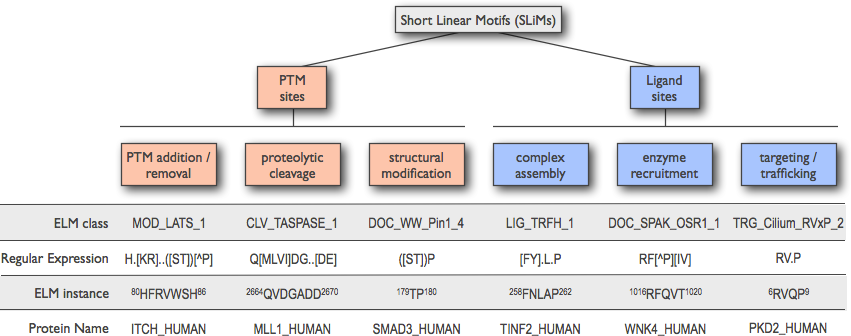
\includegraphics[width=\textwidth]{Figures/Introduction/functional_classification_of_SLiMs.png}
\caption{
\textbf{Figure functional\_classification\_of\_SLiMs} For each ELM class, the
functional category to which it belongs is indicated by a three-letter prefix.
Each ELM class is defined by a regular expression. Peptide sequences in
proteins that match the regular expression of a specific ELM class and that
were experimentally validated to be functional motifs are captured as ELM
instances of that class. Degrons are a specific subtype of enzyme-recruiting
docking motifs (see text for a detailed description).
}
\end{figure}

\subsection*{Critical Parameters and
Troubleshooting}\label{critical-parameters-and-troubleshooting}

\emph{instructions: optionally 2 separate sections.}

\section*{Internet Resources with
Annotations}\label{internet-resources-with-annotations}

http://www.clustal.org/omega Clustal Omega (\cite{21988835}) is a tool
for the alignment of multiple nucleic acid and protein sequences.

http://www.jalview.org Jalview (\cite{19151095}) is a Java desktop
application (and browser applet) that employs web services for sequence
alignment and visualization.

http://proviz.ucd.ie ProViz (\cite{27085803}) is an interactive protein
exploration tool, which searches several databases for information about
a given query protein. Data relevant to the protein like an alignment of
homologues, linear motifs, post translational modifications, domains,
secondary structure, sequence variations and others are graphically
represented relative to their position in the protein.
